\documentclass[aspectratio=169, 8pt, xcolor={svgnames}, hyperref={linkcolor=black}]{beamer}
\usepackage[labelfont={color=amethyst,bf}]{caption}
\setbeamercolor{background canvas}{bg=white}
\usetheme[progressbar=frametitle]{metropolis}
\usepackage{appendixnumberbeamer}
\usepackage{url}
\usepackage{booktabs}
\usepackage{braket}
\usepackage[scale=2]{ccicons}
\usepackage{amsfonts}
\usepackage{amssymb}
\usepackage[english]{babel}
\colorlet{col1}{teal}
\colorlet{col2}{yellow}
\colorlet{col3}{green}
\usepackage{fontawesome}
\usepackage{subcaption}
\usepackage{multicol}
\usepackage{bm}
\usepackage{algorithm}
\usepackage{overpic}
\usepackage{algpseudocode}
\usepackage{enumitem}

\usepackage[]{pseudo}


\usepackage{tikz}
\usetikzlibrary{positioning,arrows,calc,math,angles,quotes}
\usepackage{blochsphere}


\usetikzlibrary{arrows,automata}
\usetikzlibrary{positioning}
\usetikzlibrary{arrows.meta,
                bending,
                intersections,
                quotes,
                shapes.geometric}

\tikzset{
    state/.style={
           rectangle,
           rounded corners,
           draw=black, very thick,
           minimum height=1em,
           inner sep=2pt,
           text centered,
           },
}


\definecolor{myv}{rgb}{0.36, 0.22, 0.33}
\definecolor{gio}{rgb}{0.45, 0.31, 0.59}
\definecolor{light}{rgb}{0.8, 0.8, 1}
\definecolor{warmblack}{rgb}{0.0, 0.26, 0.26}
\definecolor{brown(web)}{rgb}{0.65, 0.16, 0.16}
\definecolor{cadmiumgreen}{rgb}{0.0, 0.42, 0.24}
\definecolor{darkmidnightblue}{rgb}{0.0, 0.2, 0.4}
\definecolor{brightube}{rgb}{0.82, 0.62, 0.91}
\definecolor{carnelian}{rgb}{0.7, 0.11, 0.11}
\definecolor{codegreen}{rgb}{0,0.6,0}
\definecolor{codegray}{rgb}{0.5,0.5,0.5}
\definecolor{codepurple}{rgb}{0.58,0,0.82}
\definecolor{backcolour}{rgb}{0.95,0.95,0.92}
\definecolor{amethyst}{rgb}{0.6, 0.33, 0.73}

\definecolor{light-gray}{gray}{0.95}
\newcommand{\code}[1]{\colorbox{light-gray}{\texttt{#1}}}


\usepackage{listings}
\lstdefinestyle{mystyle}{
    backgroundcolor=\color{backcolour},
    commentstyle=\color{codegreen},
    keywordstyle=\color{codepurple},
    numberstyle=\tiny\color{codepurple},
    stringstyle=\color{magenta},
    basicstyle=\footnotesize,
    breakatwhitespace=false,
    breaklines=true,
    captionpos=b,
    keepspaces=true,
    numbers=left,
    numbersep=5pt,
    showspaces=false,
    showstringspaces=false,
    showtabs=false,
    tabsize=2
}

\lstset{style=mystyle}
\usepackage[most]{tcolorbox}
\usepackage{xcolor}


%\usepackage[citecolor = green, linkcolor = blue, bookmarks=true, urlcolor=blue,
%colorlinks=true, pagebackref=true]{hyperref}


%\usepackage{xspace}

\title{Grover search algorithm}
\subtitle{Quantum Computing Minicourse ICTP-SAIFR}
\date{8 April 2024}
\author{Stefano Carrazza$^\ddag$ and Matteo Robbiati$^\dagger$}
\institute{$^\ddag$ Associate Professor \& Researcher, University of Milan and INFN Milan, Italy.\\
$^\dagger$ PhD candidate, University of Milan, Italy and CERN, Switzerland.}


\begin{document}

\begin{frame}
\maketitle
\begin{picture}(0,0)
    \put(270,40){
        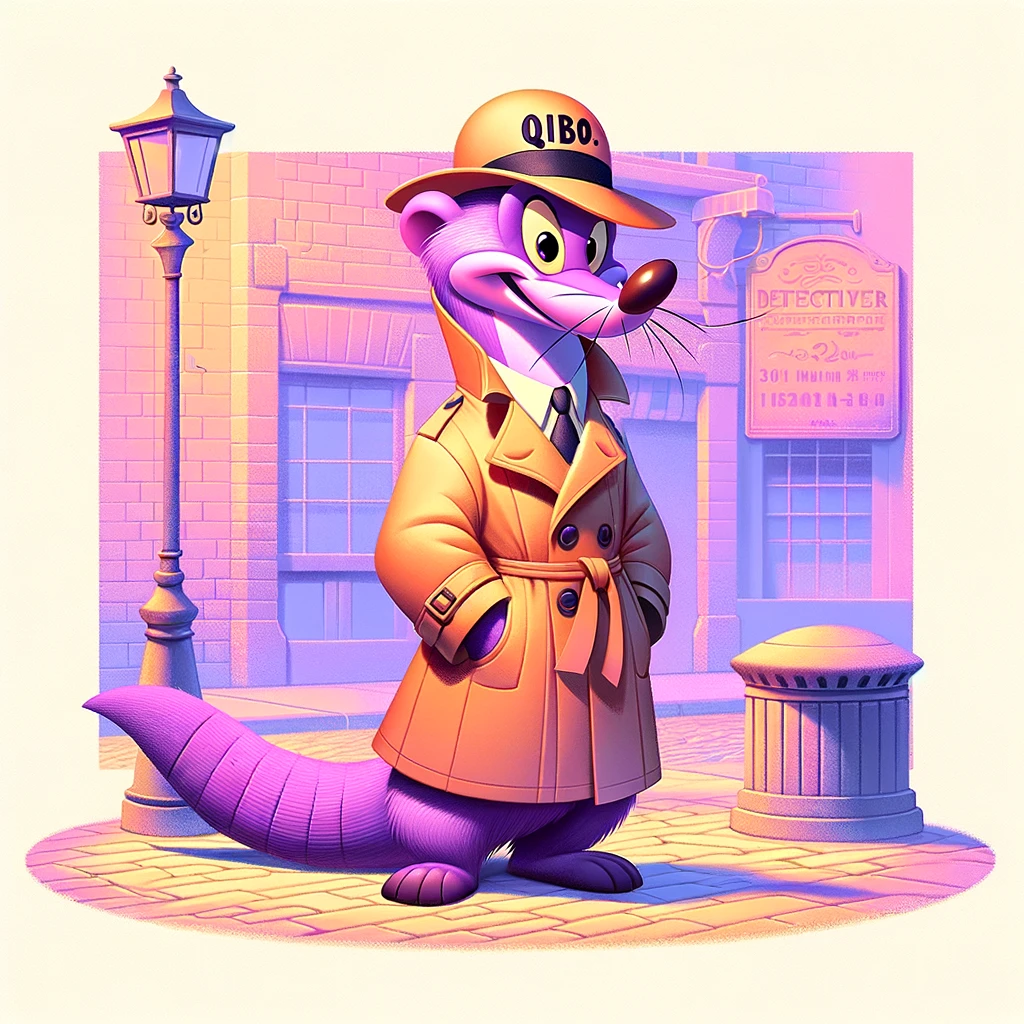
\includegraphics[width=0.25\textwidth]{figures/qibo_detective.png}
    }
\end{picture}
\end{frame}

\begin{frame}{Motivation}
The Grover algorithm is powerful when searching an item
among an unordered set of candidates.

\begin{multicols}{3}
Extract the jack of clubs from a Poker deck
\begin{figure}
    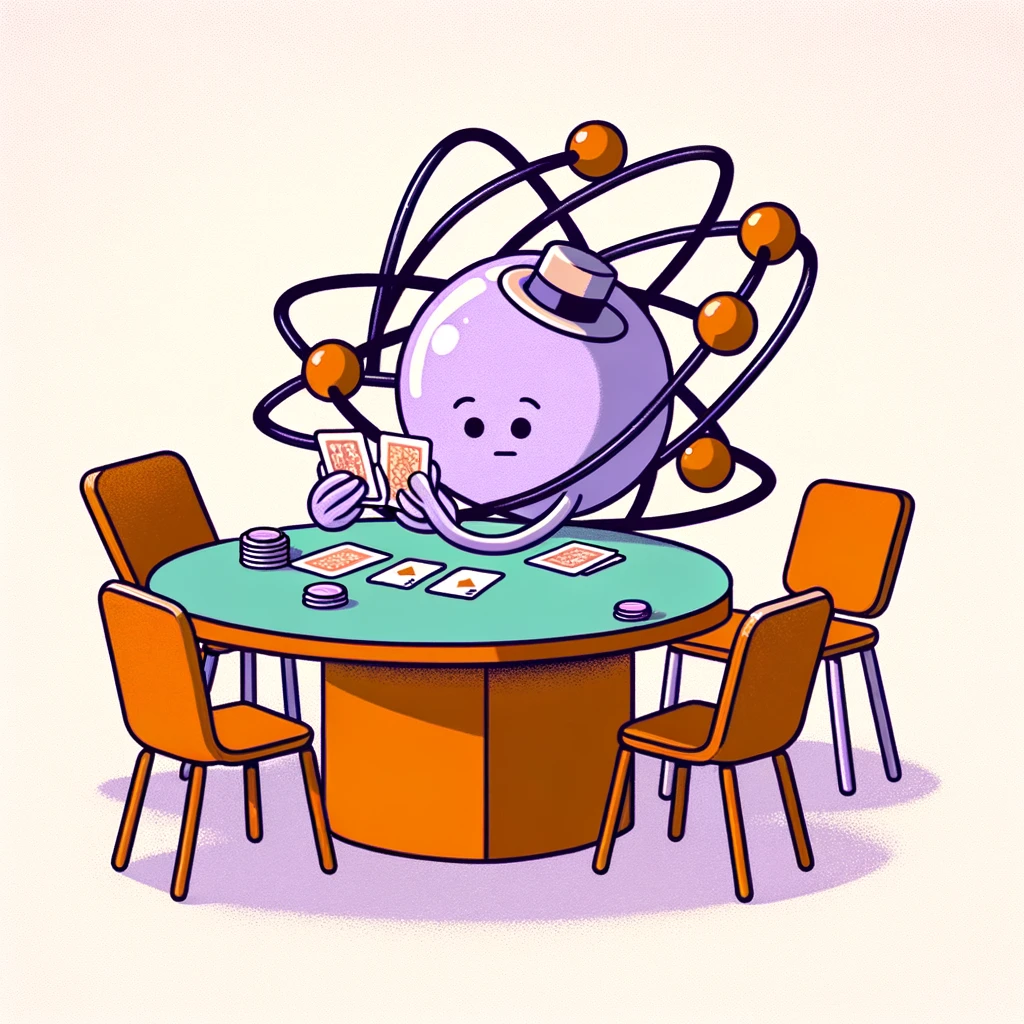
\includegraphics[width=.25\textwidth]{figures/poker.png}
\end{figure}

Find a passcode composed of 10 numbers
\begin{figure}
    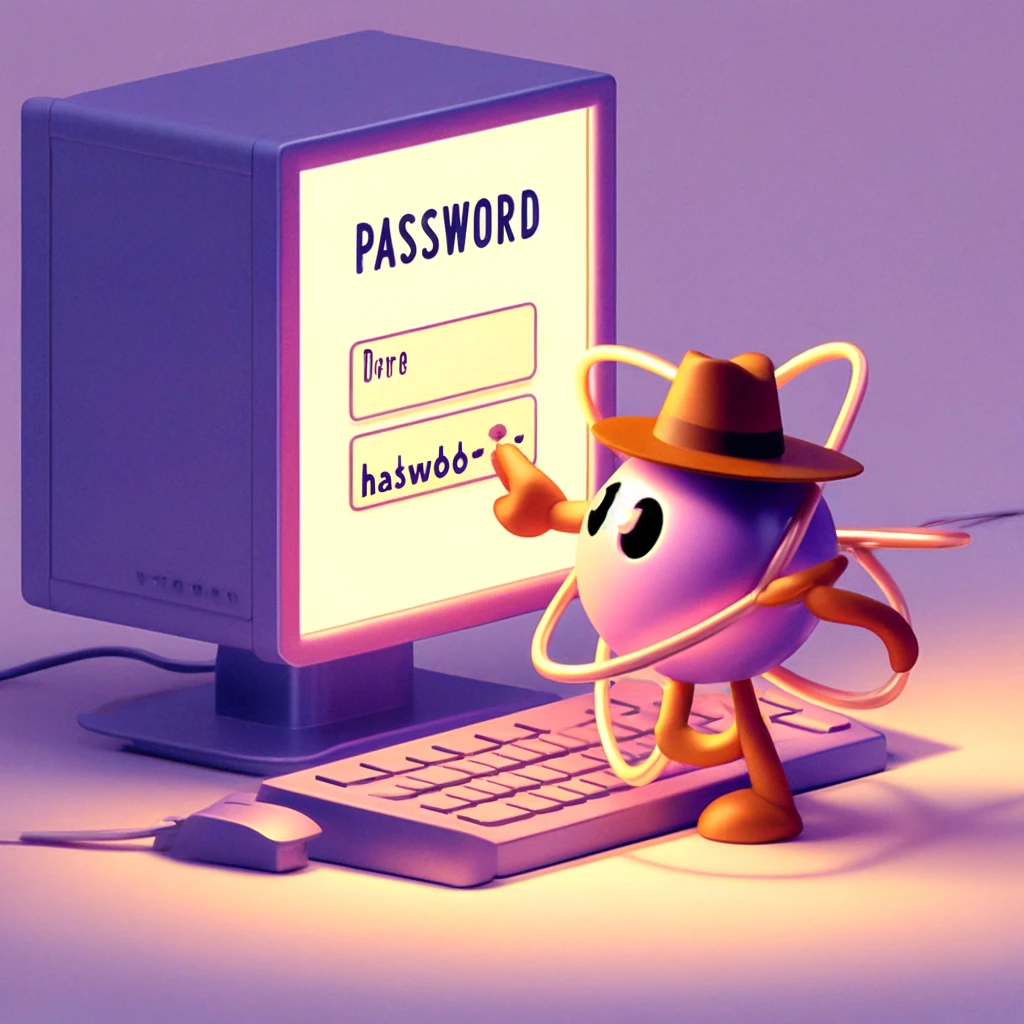
\includegraphics[width=.25\textwidth]{figures/pwd.png}
\end{figure}

Find an antidote to the Cobra poison, exploring $10^{20}$
molecules
\begin{figure}
    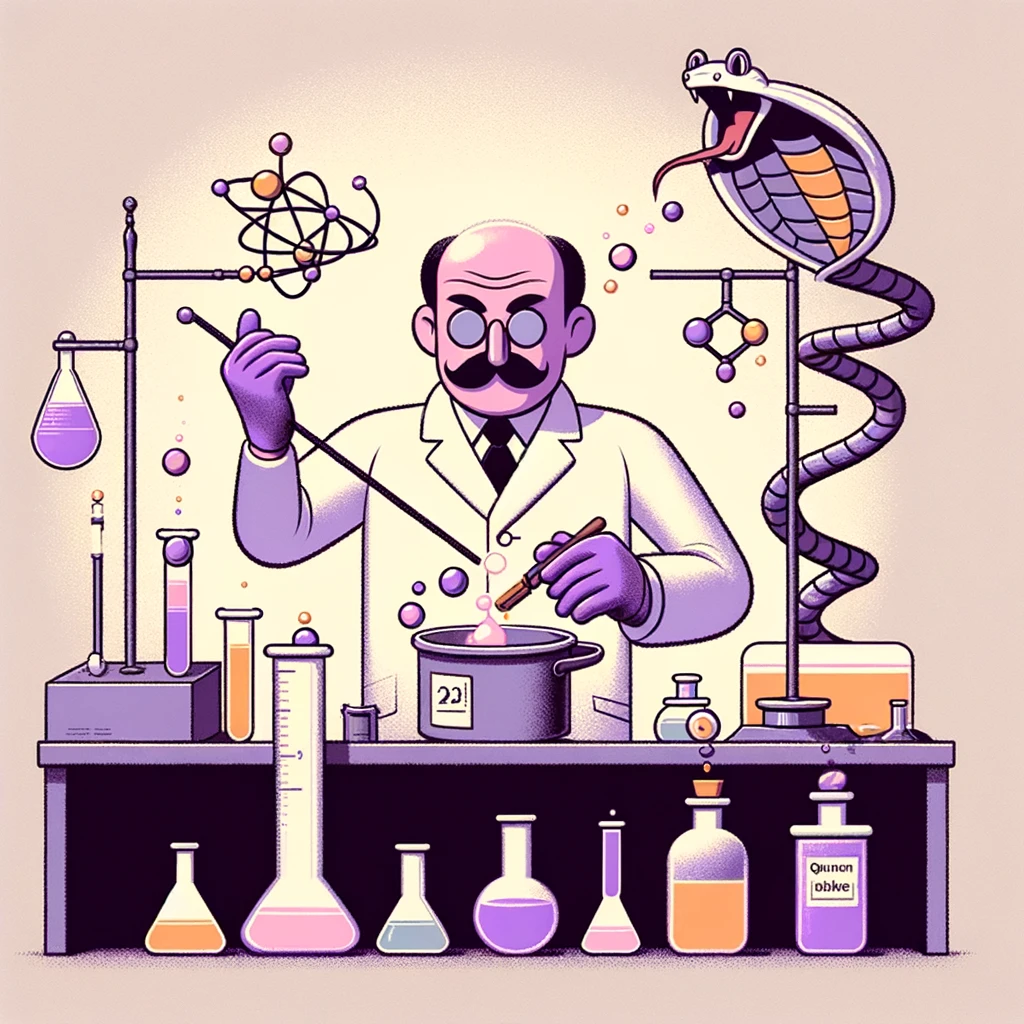
\includegraphics[width=.25\textwidth]{figures/cobra.png}
\end{figure}
\end{multicols}

\faQuestion\,\,How many attempts could you need, in the worst scenario, to explore all the possibilities?

\faExclamationTriangle\,\, In the worst scenario, you will need to check \textbf{$52$ cards}, \textbf{$10^{10}$} \textbf{passcodes}
and \textbf{$10^{20}$} \textbf{molecules}.
\end{frame}

\begin{frame}{Quadratic speedup}
If we consider a time cost of $\delta=10^{-8}$ seconds for any algorithmic call (quantum or classical) we would wait:
\begin{multicols}{2}
\textbf{On a classical computer}
\begin{itemize}[noitemsep]
\item[\footnotesize\faCircle] $0.52\,\,\mu \text{s}$ to find the jack of clubs;
\item[\footnotesize\faCircle] $100$ seconds to find the passcode;
\item[\footnotesize\faCircle] $\sim 31688$ years to find the Cobra antidote.
\end{itemize}
\begin{figure}
    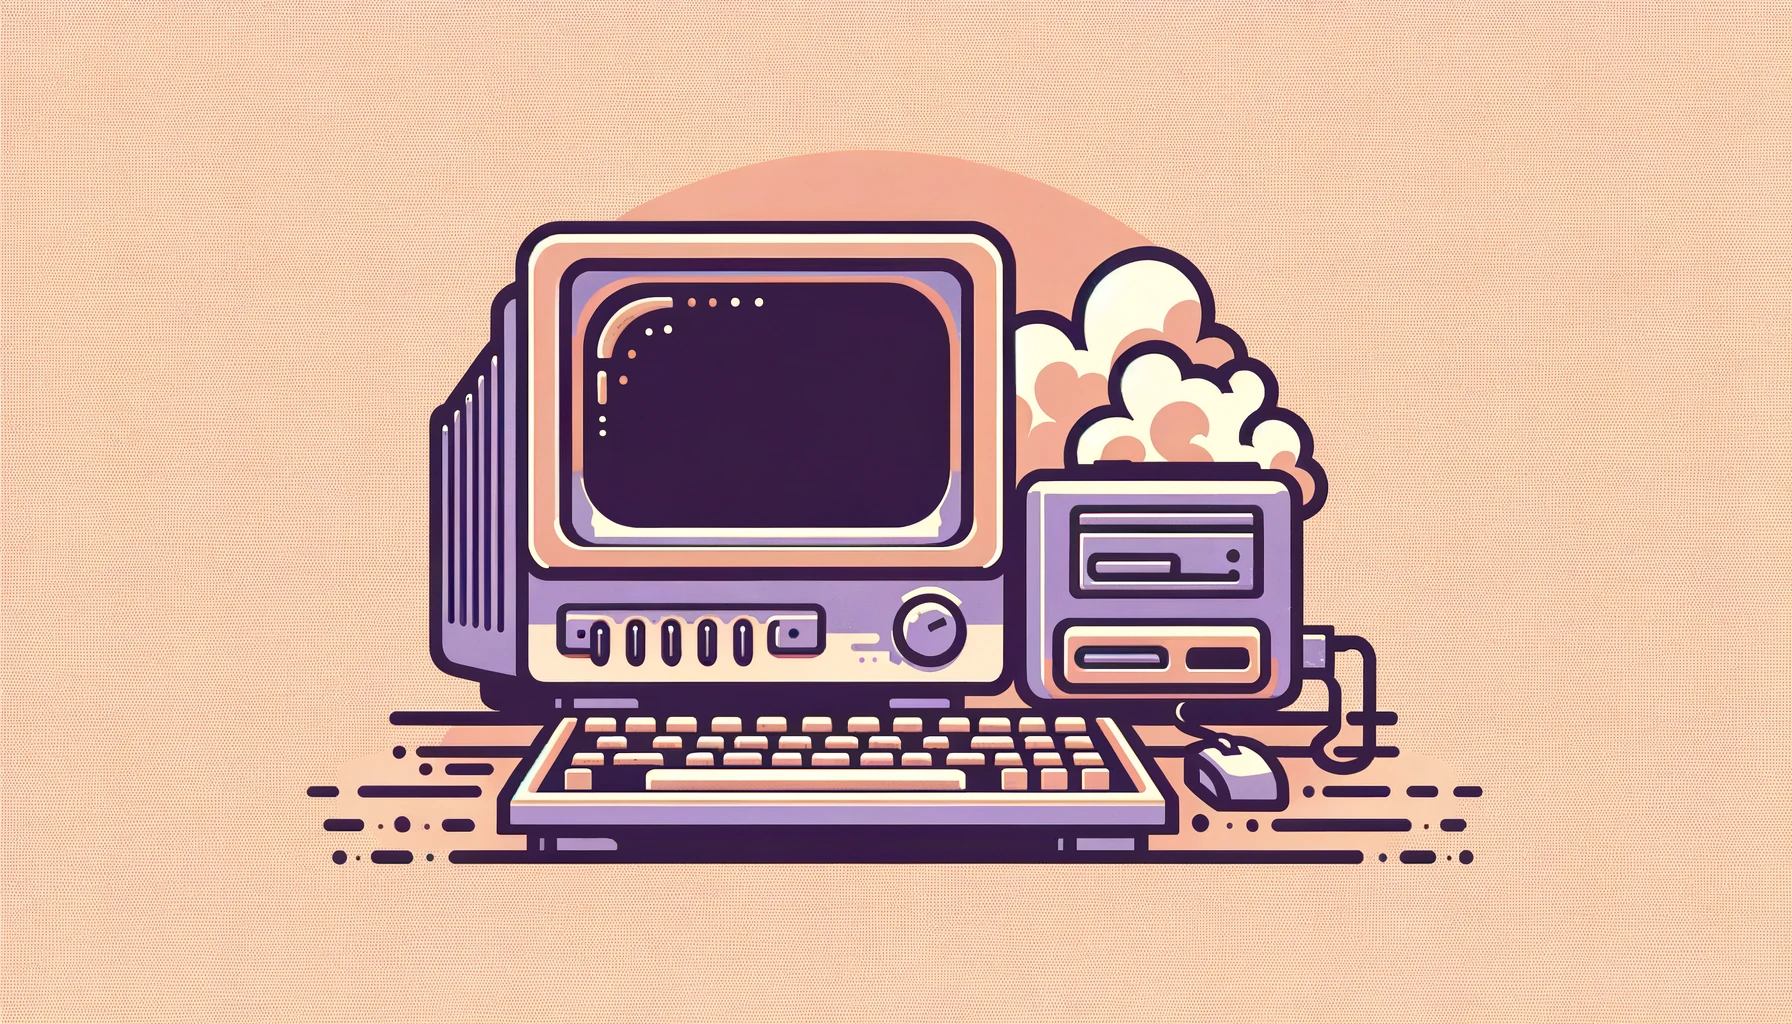
\includegraphics[width=.35\textwidth]{figures/ccomp.png}
\end{figure}

\textbf{On a quantum computer}
\begin{itemize}[noitemsep]
\item[\footnotesize\faCircle] $0.0721\,\,\mu \text{s}$ to find the jack of clubs;
\item[\footnotesize\faCircle] $0.001$ seconds to find the passcode;
\item[\footnotesize\faCircle] $100$ seconds to find the Cobra antidote.
\end{itemize}
\begin{figure}
    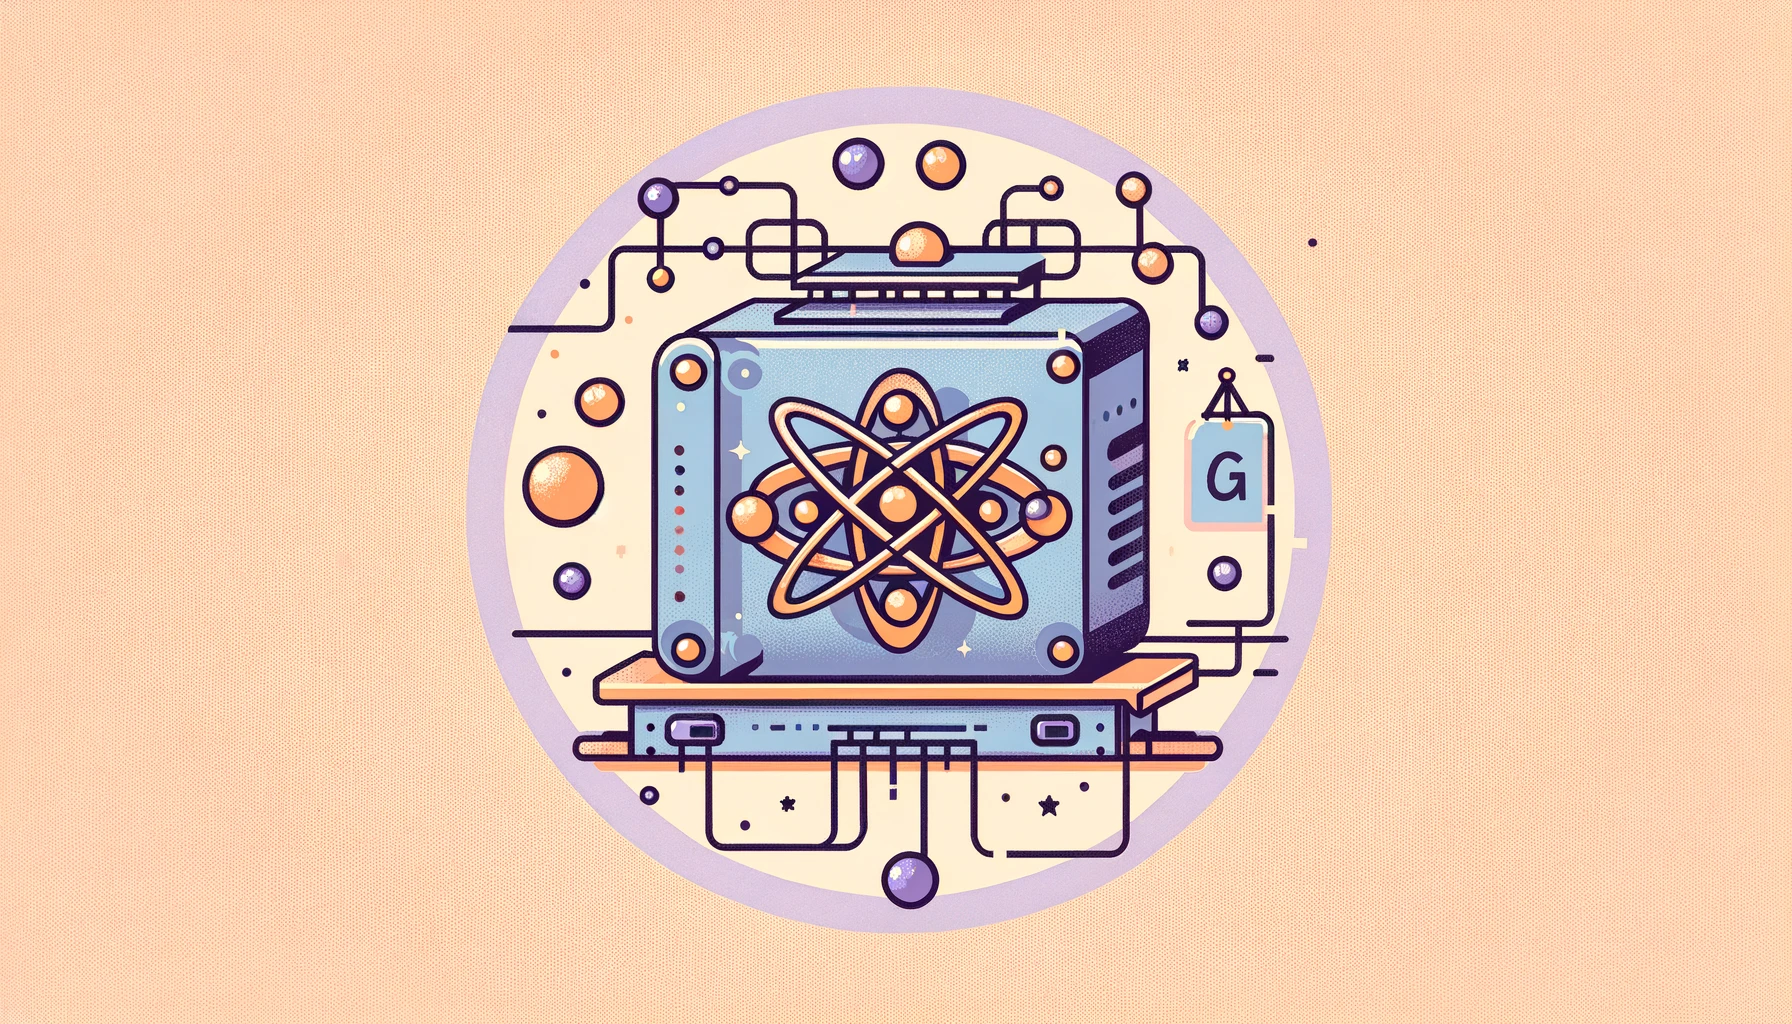
\includegraphics[width=.35\textwidth]{figures/qcomp.png}
\end{figure}
\end{multicols}
\begin{tcolorbox}[colback=red!15]
The Grover algorithm solves this kind of search with a number of algorithmic calls
proportional to $\sqrt{N}$, where $N$ is the dimension of the search space.
\end{tcolorbox}
\end{frame}


\begin{frame}{The Grover algorithm}
We consider a system of $N+1$ qubits: the system plus one ancilla. One of the $M=2^N$ components of the system's
state, which we call $\ket{\omega}$, will represent the item we are searching for.

\begin{itemize}[noitemsep]
\item[1.] prepare the system of $N$ qubits into the maximally superposed state;
\item[2.] prepare the ancilla qubit into the $\ket{-}$ state;
\item[3.] apply the Grover operator, which is able to detect $\omega$ among the components
and to amplify its amplitude;
\item[4.] repeat 3. for the optimal number of times;
\item[5.] perform the measurements on the system qubits: the target component $\ket{\omega}$
will come out with probability close to one.
\end{itemize}
\pause

In terms of quantum circuit:
\begin{figure}
    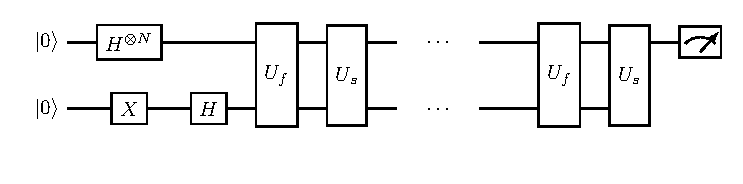
\includegraphics[width=.9\textwidth]{figures/grover-circ.pdf}
\end{figure}


\end{frame}

\begin{frame}{step 1 and 2: the state preparation}
We consider a set of $M=2^{N}$ unordered items and we encode them into the state of
an $N$ qubits system:
$$
\begin{bmatrix}
\text{item}_1 \\
\text{item}_2 \\
\dots \\
\text{item}_{2^N}
\end{bmatrix} \qquad \to \qquad
\ket{\psi} = \begin{bmatrix}
\psi_{00 \dots 0} \\
\psi_{00 \dots 1}  \\
\dots \\
\psi_{11 \dots 1}
\end{bmatrix}
\equiv
\begin{bmatrix}
x_1 \\
x_2  \\
\dots \\
x_M
\end{bmatrix} .
$$
\pause

We make use of an ancilla qubit too. The state of the system is then: $\ket{x}_N \ket{y}$. \pause

In this framework, the target solution $\omega$ is represented by one of the components of $\ket{x}_N$. \pause

The first step of the algorithm is the state preparation into the following superposed state:
\begin{multicols}{2}
$$ H^{\otimes N} \ket{0}_N \otimes HX \ket{0} = \biggl[ \frac{1}{M}\sum_{i=1}^{M} \ket{x_i} \biggr] \otimes \ket{-} = \ket{s}\otimes \ket{-}. $$
\textcolor{carnelian}{We move the system state from the computational zero
to the maximally superposed state $\ket{s}$.}

\begin{figure}
   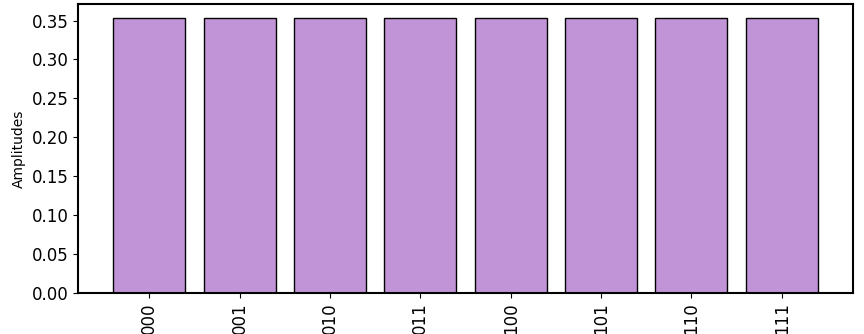
\includegraphics[width=0.5\textwidth]{figures/state1.png}
   \caption*{Amplitudes of $\ket{x}_N$ with $N=3$ and $\ket{\omega} = \ket{001}$}
\end{figure}
\end{multicols}

\end{frame}

\begin{frame}{Step 3: the oracle $U_f$}
We consider now a function $f:\{0,1\}^N \to \{0,1\}$ which can detect the correct solution $\ket{\omega}$:
$$
f(x) = \begin{cases}
1 \qquad \text{if\,\,} x=\omega, \\
0 \qquad \text{otherwise}.
\end{cases} $$ \pause
This function is typically embedded into a quantum oracle $U_f$ which is able to
recognize the solution for us. It's important to underline that even if the oracle
can detect the solution, may don't know it's exact value. \pause

\textcolor{carnelian}{The oracle marks the solution (one of the amplitudes) by flipping its sign thanks to
a phase-kickback procedure.} \pause


\begin{multicols}{2}
In practice, this can be done by setting up a multi-controlled operation
which applies a phase kickback only if the control state is $\ket{\omega}$.
$$ U_f \ket{x}\ket{-} = (-1)^{f(x)}\ket{x}\ket{-}. $$
Its action on $\ket{\omega}$ is:
$$ U_f \ket{\omega}\ket{-} = -\ket{\omega}\ket{-}. $$
where $f(x)$ follows the rule exposed before.
\begin{figure}
   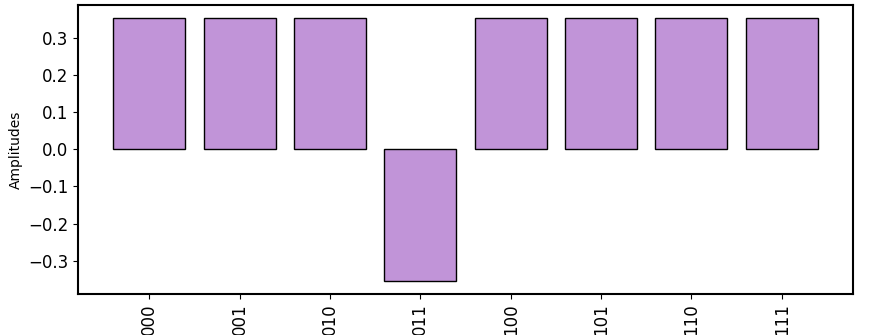
\includegraphics[width=0.5\textwidth]{figures/state2.png}
   \caption*{Amplitudes of $\ket{x}_N$ with $N=3$ and $\ket{\omega} = \ket{001}$}
\end{figure}
\end{multicols}

\end{frame}

\begin{frame}{Step 4: the diffusion operator $U_s$}
Now $\ket{\omega}$ is marked. We need to amplify its amplitude so that we can
detect it among the $M$ components of $\ket{x}$. \pause

To this purpose, we introduce the diffusion operator
$$ U_s =  2 \ket{s}\bra{s} - I, $$
whose action is a reflection of the system with respect to the state:
$$ \ket{s} = \frac{1}{2^{M}}\sum_{i=1}^{M} \ket{x_i}. $$ \pause

Since the amplitude of $\ket{\omega}$ was flipped by $U_f$, the action of $U_s$
will produce an increasing of $\ket{\omega}$ and, consequently, a decreasing of the
other components. \pause

\begin{multicols}{2}
\textit{\\}
$U_s$ is also known as \textcolor{carnelian}{``inversion by the mean"}, in fact, it can be shown
it implements an inversion w.r.t. the mean value of the amplitudes of $\ket{x}$.
\begin{figure}
   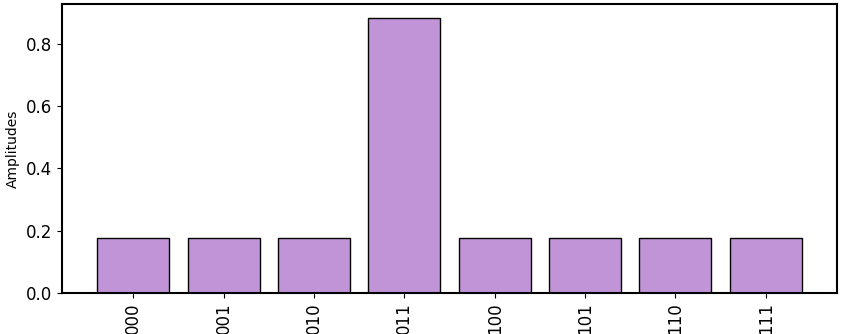
\includegraphics[width=0.5\textwidth]{figures/state3.png}
   \caption*{Amplitudes of $\ket{x}_N$ with $N=3$ and $\ket{\omega} = \ket{001}$}
\end{figure}
\end{multicols}
\end{frame}

\begin{frame}{Graphical intuition}
We can visualize the Grover's action using vectors.
\begin{figure}
   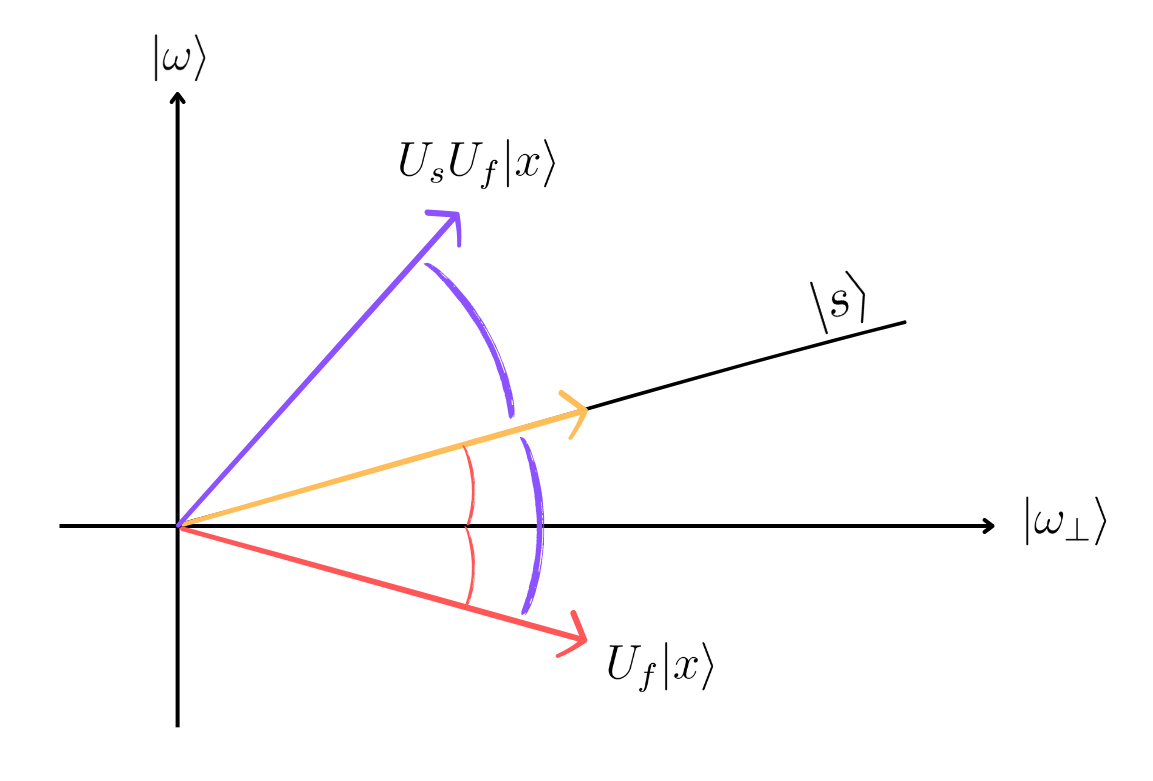
\includegraphics[width=0.6\textwidth]{figures/vectors.png}
\end{figure}
We are iteratively moving the system state through the target $\ket{\omega}$.
\end{frame}

\begin{frame}{How many times do we need to iterate Grover?}
As we can deduce from the previous slide, there exist an \textbf{optimal number} of Grover iterations fixed by geometry.

\begin{itemize}
\item[1.] we can decompose $\ket{x}$ into the \textit{winning} and the \textit{losing}
components $\ket{s} = \sqrt{\frac{1}{M}} \ket{\omega} + \sqrt{\frac{M-1}{M}} \ket{\omega_{\bot}}.$
\item[2.]  The same vector can be
defined in terms of the angle in the plane: $\,\ket{s} = \sin \theta \ket{\omega} + cos \theta \ket{\omega_{\bot}}.$
\end{itemize}
\begin{multicols}{2}
\begin{itemize}
\item[3.] from 1. and 2. we can write $\theta = \text{arcsin}\bigl(1/\sqrt{M}\bigr)$ and, if $M$ is large,
$\theta \approx 1/\sqrt{M}. $
\item[4.] the action of $U_s U_f$ on $\ket{x}$ is equal to a rotation of $2\theta$ of the vector.
\item[5.] after $k$ iteration of Grover, the angle has become: $\alpha = (2k + 1)\,\theta$, and, to maximize $\sin \alpha$:
$$ \alpha = \frac{\pi}{2} \quad \to \quad k = \frac{\pi}{4\theta} - \frac{1}{2} = \frac{\pi}{4} \sqrt{M} - \frac{1}{2}. $$
\item[6.] from 5. we need to get an integer, since we are talking about iterations.
Commonly $\theta \approx \frac{\pi}{4} \sqrt{M}.$
\end{itemize}
\begin{figure}
   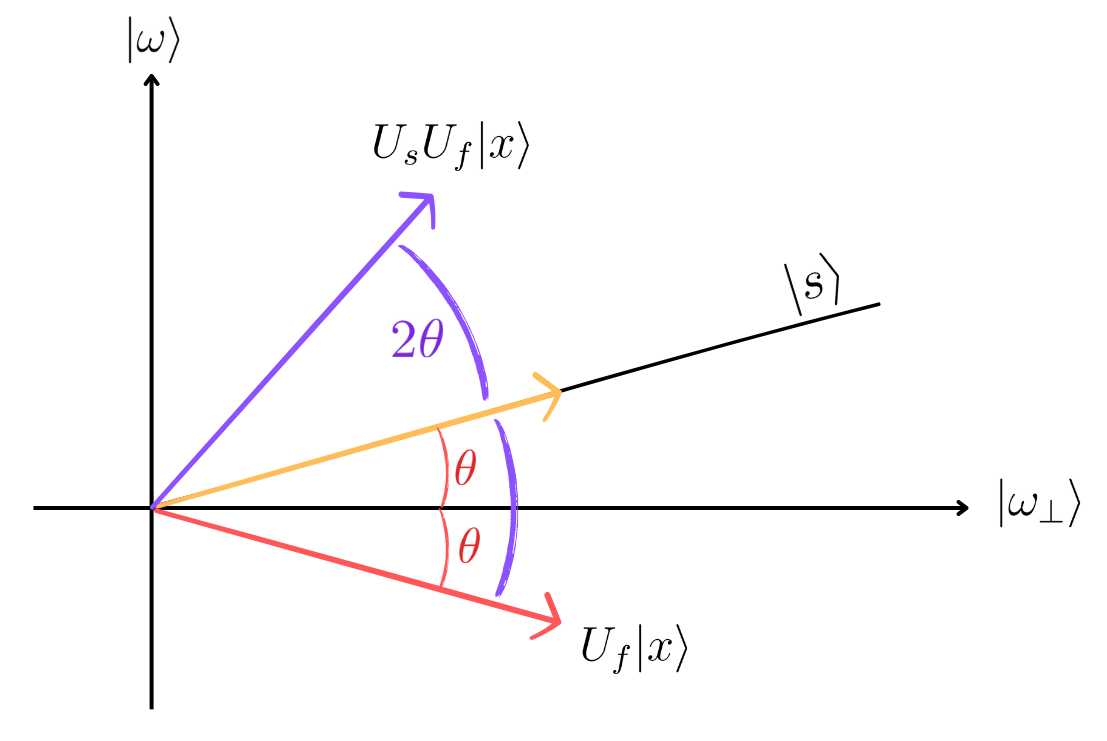
\includegraphics[width=0.5\textwidth]{figures/thetas.png}
\end{figure}
\end{multicols}
\end{frame}

\begin{frame}
\centering
\Huge Let's code!
\begin{figure}
   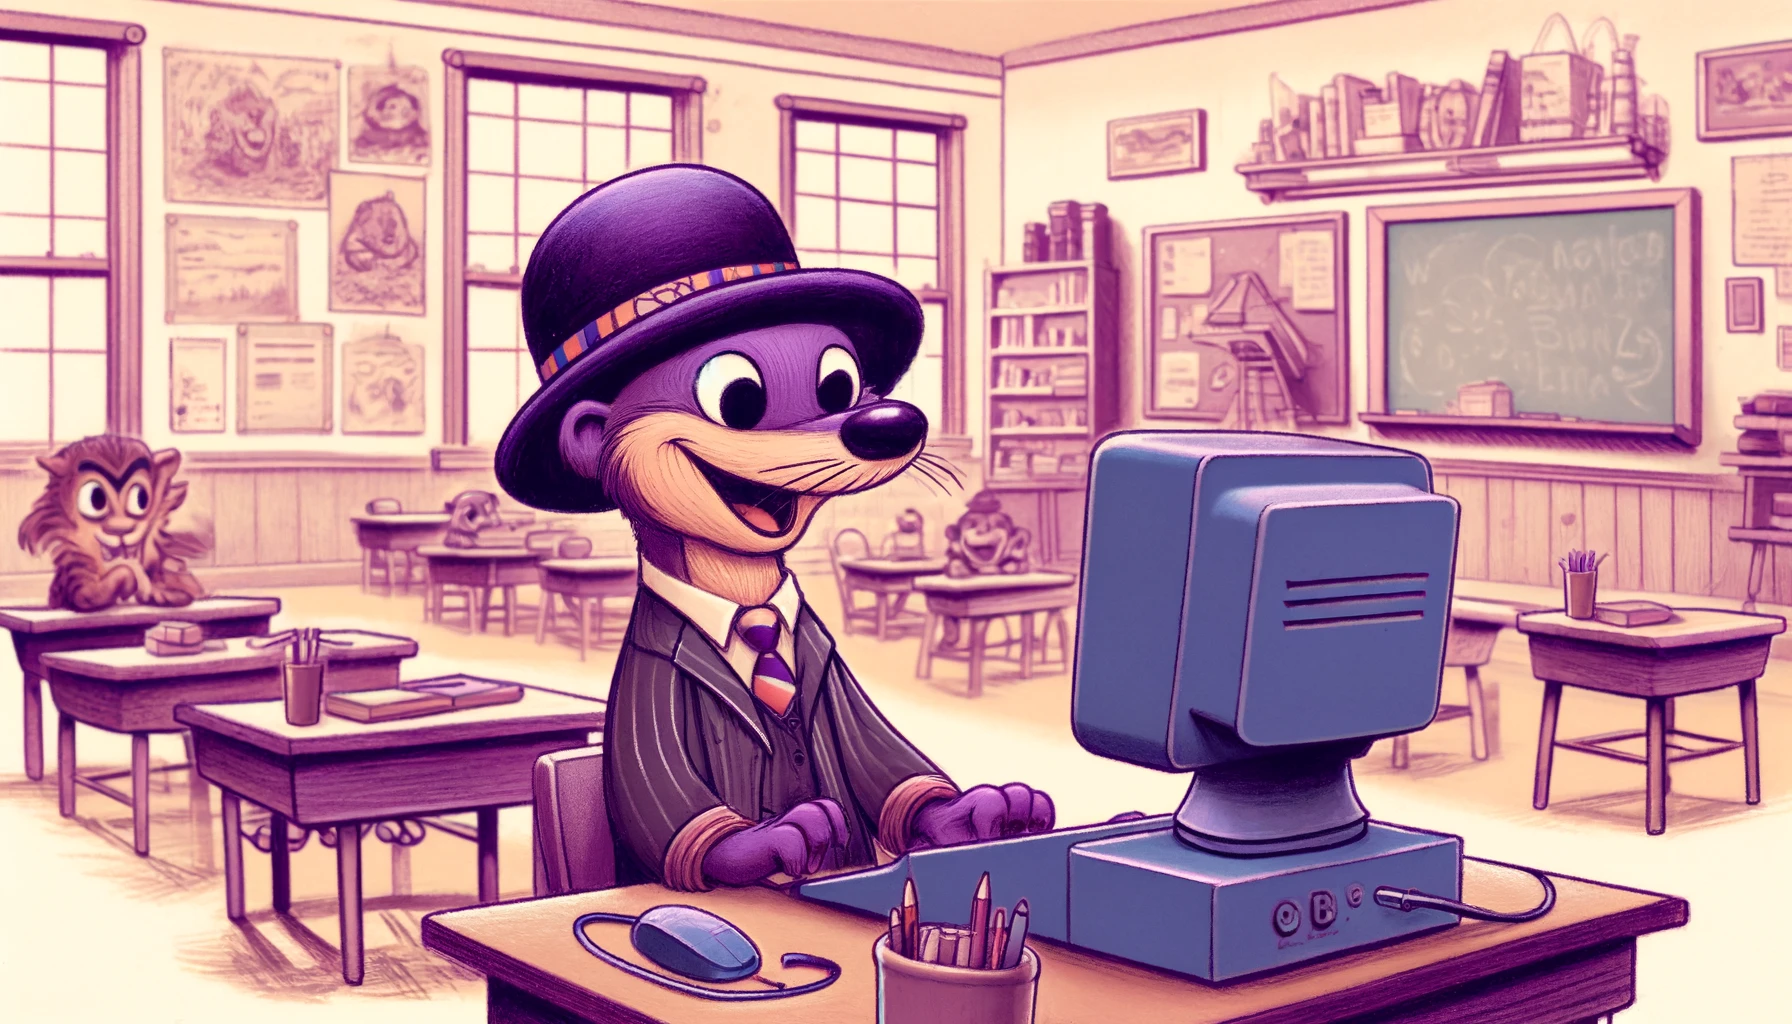
\includegraphics[width=0.7\textwidth]{figures/hands_on.png}
\end{figure}
\end{frame}

\end{document}
